\documentclass[a4paper,12pt]{article}
\usepackage{float} %здесь здесь, только здесь
%%% Работа с русским языком
\usepackage{cmap}					% поиск в PDF
\usepackage{mathtext} 				% русские буквы в формулах
\usepackage[T2A]{fontenc}			% кодировка
\usepackage[utf8]{inputenc}			% кодировка исходного текста
\usepackage[english,russian]{babel}	% локализация и переносы

%%% Дополнительная работа с математикой
\usepackage{amsmath,amsfonts,amssymb,amsthm,mathtools} % AMS
\usepackage{icomma} % "Умная" запятая: $0,2$ --- число, $0, 2$ --- перечисление

%% Номера формул
%\mathtoolsset{showonlyrefs=true} % Показывать номера только у тех формул, на которые есть \eqref{} в тексте.
%\usepackage{leqno} % Нумерация формул слева

%% Свои команды
\DeclareMathOperator{\sgn}{\mathop{sgn}}

%% Перенос знаков в формулах (по Львовскому)
\newcommand*{\hm}[1]{#1\nobreak\discretionary{}
	{\hbox{$\mathsurround=0pt #1$}}{}}

%%% Работа с картинками
\usepackage{graphicx}  % Для вставки рисунков
\graphicspath{{images/}{images2/}}  % папки с картинками
\setlength\fboxsep{3pt} % Отступ рамки \fbox{} от рисунка
\setlength\fboxrule{1pt} % Толщина линий рамки \fbox{}
\usepackage{wrapfig} % Обтекание рисунков текстом

%%% Работа с таблицами
\usepackage{array,tabularx,tabulary,booktabs} % Дополнительная работа с таблицами
\usepackage{longtable}  % Длинные таблицы
\usepackage{multirow} % Слияние строк в таблице

%%% Теоремы
\theoremstyle{plain} % Это стиль по умолчанию, его можно не переопределять.
\newtheorem{theorem}{Теорема}[section]
\newtheorem{proposition}[theorem]{Утверждение}

\theoremstyle{definition} % "Определение"
\newtheorem{corollary}{Следствие}[theorem]
\newtheorem{problem}{Задача}[section]

\theoremstyle{remark} % "Примечание"
\newtheorem*{nonum}{Решение}

%%% Программирование
\usepackage{etoolbox} % логические операторы

%%% Страница
\usepackage{extsizes} % Возможность сделать 14-й шрифт
\usepackage{geometry} % Простой способ задавать поля
\geometry{top=25mm}
\geometry{bottom=35mm}
\geometry{left=35mm}
\geometry{right=20mm}
%

\usepackage{fancyhdr} % Колонтитулы
\pagestyle{fancy}
\renewcommand{\sectionmark}[1]{\markboth{#1}{}}
%\renewcommand{\headrulewidth}{0mm}  % Толщина линейки, отчеркивающей верхний колонтитул
%\lfoot{Нижний левый}
%\rfoot{Нижний правый}
%\rhead{}
%\chead{Верхний в центре}
\lhead{\thepage}
\cfoot{} % По умолчанию здесь номер страницы

\usepackage{setspace} % Интерлиньяж
%\onehalfspacing % Интерлиньяж 1.5
%\doublespacing % Интерлиньяж 2
%\singlespacing % Интерлиньяж 1

\usepackage{lastpage} % Узнать, сколько всего страниц в документе.

\usepackage{soul} % Модификаторы начертания

\usepackage{indentfirst} % Красная строка

\usepackage{soulutf8} % Модификаторы начертания

%\usepackage{hyperref}
%\usepackage[usenames,dvipsnames,svgnames,table,rgb]{xcolor}
%\hypersetup{				% Гиперссылки
%	unicode=true,           % русские буквы в раздела PDF
%	pdftitle={Заголовок},   % Заголовок
%	pdfsubject={Тема},      % Тема
%	pdfcreator={Создатель}, % Создатель
%	pdfproducer={Производитель}, % Производитель
%	pdfkeywords={keyword1} {key2} {key3}, % Ключевые слова
%	colorlinks=true,       	% false: ссылки в рамках; true: цветные ссылки
%	linkcolor=red,          % внутренние ссылки
%	citecolor=green,        % на библиографию
%	filecolor=magenta,      % на файлы
%	urlcolor=cyan           % на URL
%}

%\renewcommand{\familydefault}{\sfdefault} % Начертание шрифта

\usepackage{multicol} % Несколько колонок

\author{\LaTeX{} в Вышке}
\title{3.2 Оформление документа в целом}
\date{\today}

\begin{document} % конец преамбулы, начало документа
	\thispagestyle{empty}
	\begin{center}
		\textit{Федеральное государственное автономное образовательное\\ учреждение высшего образования }
		\vspace{0.5ex}
		
		\textbf{«Московский физико-технический институт\\ (национальный исследовательский университет)»}
	\end{center}
	\vspace{10ex}
	%\begin{flushright}
	%	\noindent
	%	\textit{Фамилия Имя Отчество}
	%	\\
	%	\textit{студент факультета экономики \\(группа 211И)}
	%\end{flushright}
	\begin{center}
		\vspace{13ex}
		\so{\textbf{Лабораторная работа №2.1.2}}
		\vspace{1ex}
		
		по курсу общей физики
		
		
		на тему:
		
		\textbf{\textit{<<Определение $C_p/C_v$ методом \\ адиабатического расширения газа>>}}
		\vspace{30ex}
		\begin{flushright}
			\noindent
			\textit{Работу выполнил:}
			\\
			\textit{Баринов Леонид \\(группа Б02-827)}
		\end{flushright}
		\vfill
		Долгопрудный \\2019
	\end{center}
	\newpage
	\setcounter{page}{1}
	\section{Аннотация}
	\fancyhead[R]{\nouppercase{\leftmark}}
	В работе будет определено отношение $C_p/C_v$ для воздуха по измерению давления в стеклянном сосуде.
	\section {Теоритические сведения}
	\subsection{Адиабатический процесс}
	Процесс, происходящий без теплообмена с окружающей средой, называется адиабатическим. Получим уравнение такого процесса для идеального газа, внутренняя энергия которого $U$ не зависит от объёма.
	
	Из первого начала термодинамики при $\delta Q = 0$ для идеального газа, у которого $dU = C_v dT$, получим $C_v dT + P dV = 0$. Исключим отсюда давление $P$ c помощью уравнения состояния $PV = RT$:
	\[C_V\frac{dT}{T}+R\frac{dV}{V} = 0 \]
	
	При постоянной величине $C_v$, что соответствует классической теории теплоемкости, уравнение легко интегрируется:
	\[TV^{R/C_v} = TV^{\gamma - 1} = \text{const} \]
	
	Это уравнение адиабатического процесса в переменных $T, V$. Преобразуем его к переменным $P, V$. Снова используя $PV = RT$, а также соотношение Майера, получим уравнение, которое называется также адиабатой Пуассона:
	\begin{equation}
	PV^{\gamma} = \text{const}
	\end{equation}
	Здесь $\gamma$ -- показатель адиабаты, играющий важную роль при описании адиабатических процессов.
	\begin{equation}
	\gamma = \frac{C_p}{C_v}
	\end{equation}
	\section{Оборудование}
	В работе используются: стеклянный сосуд; $U$--образный жидкостный манометр; резиновая груша; газгольдер с углекислым газом.
	\subsection{Экспериментальная установка}
	Используемая для опытов установка состоит из стеклянного сосуда $\text{А}$ (объемом около 20 л), снабженного краном $\text{К}$, и $U$--образного жидкостного манометра, измеряющего избыточное давление газа в сосуде. Схема установки показана на рисунке 1.
	
	Избыточное давление воздуха создается с помощью резиновой груши, соединенной с сосудом трубкой с краном $\text{К}_1$. 
	\begin{figure}[H]
		\begin{center}
			\includegraphics[width=0.7\linewidth]{1}
			\caption{Установка для определения $C_p/C_v$ методом адиабатического расширения газа}
		\end{center}
	\end{figure}

В начале опыта в стеклянном сосуде $\text{А}$ находится исследуемый газ при комнатной температуре $T_1$ и давлении $P_1$, несколько превышающем атмосферное давление $P_0$. После открытия крана $\text{К}$, соединяющего сосуд $\text{А}$ с атмосферой, давление и температура газа будут понижаться. Это уменьшение температуры приближенно можно считать адиабатическим. Приближение основано на том, что равновесие в газах по давлению устанавливается намного быстрее, чем равновесие по температуре, которое происходит в процессе «диффузии тепла», диффузии интенсивности хаотического движения. Поэтому
\begin{equation}
\Delta t_P \ll \Delta t_T
\end{equation}
где $\Delta t_P$ и $\Delta t_T$ обозначают соответственно времена выравнивания давления и температуры.

Выполнение условия (1) зависит, конечно, и от конструкции установки, в частности, от величины отверстия в кране $\text{К}$, которое должно быть достаточно большим. Ниже приведены численные оценки величин $\Delta t_P$ и $\Delta t_T$ и их влияния на точность опытов. Если открыть кран $\text{К}$ в течение такого промежутка времени $\Delta t$, что удовлетворяются условия
\begin{equation}
\Delta t_P \ll \Delta t \ll \Delta t_T
\end{equation}
то теплообменом через стенки баллона можно приближенно пренебречь и считать процесс адиабатическим.

Преобразуем уравнение адиабаты (1) с помощью уравнения Клапейрона к переменным $P, T$. Обозначим состояние газа после повышения давления в сосуде и выравнивания температуры с комнатной индексом <<1>>, а состояние сразу после открытия крана и выравнивания давления с атмосферным -- индексом <<2>>. Получим
\begin{equation}
\left( \frac{P_1}{P_2} \right)^{\gamma - 1} = \left( \frac{T_1}{T_2}\right)^\gamma
\end{equation}

Давление $P_2$ после адиабатического расширения газа равно атмосферному давлению $P_0$, а температура $T_2$ будет ниже комнатной температуры $T_1$ (температура газа понижается, так как работа расширения совершается за счет внутренней энергии газа).

После того как кран $\text{К}$ вновь отсоединит сосуд от атмосферы, происходит медленное изохорическое нагревание газа со скоростью, определяемой теплопроводностью стеклянных стенок сосуда. Вместе с ростом температуры растет и давление газа. За время порядка $\Delta t_T$ система достигает равновесия, и установившаяся температура газа $T_3$ становится равной комнатной температуре $T_1$.

Изохорический процесс выравнивания температуры при закрытом кране подчиняется закону Гей-Люссака:
\begin{equation}
\frac{P_2}{T_2} = \frac{P_3}{T_3} = \frac{P_3}{T_1}
\end{equation}
Исключая с помощью (6) отношение температур $T_1/T_2$ из (5), найдем
\[ \left( \frac{P_3}{P_2} \right)^{\gamma} = \left( \frac{P_1}{P_2} \right) ^ {\gamma - 1} \]
Отсюда учитывая, что $P_2 = P_0$, находим $\gamma$:
\begin{equation}
\gamma = \frac{\ln (P_1/P_0)}{\ln (P_1/P_3)}
\end{equation}
В нашем случае давления $P_1$ и $Р_3$ отличаются от атмосферного на малую величину, измеряемую жидкостным $U$-образным манометром. Введем обозначения:
\begin{equation*}
\begin{aligned}
P_1 = P_0 + \rho g h_1, & & & & &P_3 = P_0 + \rho g h_2
\end{aligned}
\end{equation*}
Разлагая логарифмы в ряд и пренебрегая членами второго порядка малости, получим
\begin{equation}
\gamma = \frac{\ln (1 + \rho g h_1/P_0)}{\ln (1+ \rho g h_1/P_0) - \ln(1 + \rho g h_2/P_0)} \approx \frac{h_1}{h_1-h_2}
\end{equation}

Как следует из (8), для определения $\gamma$ необходимо знать избыточное (над атмосферным) давление в баллоне до адиабатического расширения газа и его избыточное давление после изохорного нагревания. Следует подчеркнуть, что обе величины должны измеряться в состоянии термодинамического равновесия, т. е. после прекращения теплообмена. Для этого необходимо закрыть кран $\text{К}$ после установления в сосуде атмосферного давления, но еще до того, когда там начнется нагревание газа. То есть нужно выполнить условия (4).

\subsection{Время вытекания газа}
Оценим время выравнивания давления $\Delta t_P$, пренебрегая вязкостью газа. В данном случае это можно сделать из-за малой длины трубки, через которую вытекает газ.

После открытия крана $\text{К}$ по газу со скоростью звука $c$ будет распространяться волна разрежения и через время $L/c$ (где $L$ — высота сосуда) она достигнет дна. Весь газ придет в движение и через несколько таких интервалов процесс вытекания будет почти установившимся, квазистационарным. При этом скорость истечения $\upsilon$ можно рассчитать по уравнению Бернулли для несжимаемой среды, поскольку давление воздуха мало отличается от атмосферного и изменением плотности допустимо пренебречь:
\[ \upsilon = \sqrt{\frac{2(P - P_0)}{\rho_0}}\]

За время $dt$ из сосуда через отверстие площадью $S_r$ вытечет масса газа $\rho_0 S_r \upsilon dt$, где плотность взята при атмосферном давлении из-за малого изменения давления газа.

В сосуде объема $V_0$ давление за это же время снизится на $dP$, и масса газа при адиабатическом истечении уменьшится на величину
\[dm = V_0 d\rho = \frac{V_0}{c^2}dP\]
Здесь использовано определение адиабатической скорости звука
\[c^2 = \left(\frac{\partial P}{\partial \rho} \right)_S \]

Составив баланс вытекающей массы и остающейся в сосуде, получим дифференциальное уравнение:
\[ \frac{dP}{\sqrt{P - P_0}} = -\frac{\sqrt{2\rho_0}S_r c^2}{V_0}dt \]
интегрируя которое, найдем искомое время вытекания газа:
\[t_P = \frac{V_0}{S_r c}\sqrt{\frac{2(P - P_0)}{\gamma P_0}}\]
Исходя из параметров установки $t_P \approx 10^{-1}\ \text{с}$. Этого достаточно, чтобы течение считать квазистационарным и применять уравнение Бернулли.

Отметим, что после выравнивания давления из-за инерции вытекающей струи могут происходить колебания воздуха в сосуде как в акустическом резонаторе. Поэтому при малых временах открытия крана $\Delta t$ (меньше одной секунды) результаты отдельных измерений заметно отличаются друг от друга (случайный разброс вызван не только колебаниями, но и неопределенностью во времени открытия крана). При увеличении времени $\Delta t$ (больше одной секунды) колебания давления из-за затухания благодаря вязкости становятся меньше, но за большее время увеличивается теплообмен. Следствием является уменьшение давления $Р_3$ и занижение значения $\gamma$.

\subsection{Нагревание газа от стенок сосуда}
В течение времени выравнивания давления ($10^{-1}\ \text{c}$) глубина прогревания невелика, значительно меньше размеров сосуда, поэтому нагревание приближенно можно считать одномерным

Все физические свойства среды, влияющие на исследуемый процесс, отражены в уравнении теплопроводности всего через один параметр — коэффициент температуропроводности $\chi = \varkappa/(\rho c_p)$, где $\varkappa$ — коэффициент теплопроводности, $c_р$ — теплоемкость при постоянном давлении единицы массы газа, $\rho$ — его плотность.

Если в начальном распределении температуры нет постоянных с размерностью длины, как, например, при нагревании полупространства от горячей стенки, то решение может быть функцией только от одного безразмерного параметра $х^2/\chi^t$, где $х$ — координата, $t$ — время (такое решение называется автомодельным). Одному и тому же значению этого параметра будет соответствовать одна и та же температура, положение которой в пространстве меняется. Расстояние от стенки до точки с любой заданной температурой увеличивается пропорционально квадратному корню из времени. При $х^2/\chi^t$ = 1, то есть при $х = \sqrt{\chi^t}$, в точном решении задачи о нагревании полупространства, температура равна примерно среднему значению между постоянной температурой горячей стенки и температурой первоначально холодной теплопроводящей среды. Это значение $х$ можно использовать для оценки толщины слоя газа, нагревшегося от стенки сосуда при предполагаемом его адиабатическом охлаждении, сопровождающим процесс вытекания.

В соответствии с оценкой времени вытекания газа из сосуда примем для определения влияния теплопроводности время $t = 0,5\ \text{с}$. Для воздуха $с_р = 0,99\ \text{Дж}/\text{(г}\cdot\text{К)}$, $p = 1,29\ \text{кг}/\text{м}^3$, $\varkappa = 2,50 \cdot 10^{-2}\ \text{Вт}/\text{(м}\cdot\text{К)}$. По этим данным $\chi = 0,19\  \text{см}^2/\text{с}$, и при $t = 0,5\ \text{с}$ глубина нагревания составит $х = 0,3\ \text{см}$.

При радиусе сосуда $R = 12,5\ \text{см}$ доля неохлажденного воздуха из- за контакта со стенкой сосуда составит, согласно приведенной оценке, $2\pi Rx/(\pi R^2) = 0,05$, то есть $5\%$ от массы газа в сосуде. Следовательно, давление $P_3$ и величина $h_2$ будут во столько же раз меньше, что приведет к уменьшению величины $\gamma$ в соответствии с формулой (8) в $h_2/(h_1 - h_2) \cdot 0,05$ раз. Приведенная оценка ошибки может быть несколько уменьшена, если учесть охлаждение стеклянных стенок сосуда.

\subsection{Охлаждение стенок}

Глубину охлаждения стенок сосуда за время вытекания газа можно оценить аналогичным способом.

Для стекла теплоемкость $c = 1,0\ \text{кДж}/\text{(кг}\cdot \text{К)}$, плотность $р = 2,5\cdot10^3\ \text{кг}/\text{м}^3$, теплопроводность $\varkappa = 1,0\ \text{Вт}/\text{(м}\cdot \text{К)}$. По этим данным получим $\chi = 0,4 * 10^{-2}\ \text{см}^2/\text{с}$ и глубина охлаждения получится равной всего $0,045\ \text{см}$.

Из полученной оценки следует, что глубина охлаждения стекла примерно в семь раз меньше, чем глубина нагревания воздуха за то же время. Если учесть, что теплоемкость стекла на единицу объема на три порядка больше теплоемкости воздуха, то получится, что изменение температуры стенок будет примерно в сто раз меньше, чем у газа. Оценка ошибки остается прежней, учет охлаждения стекла в данном случае не оказывает заметного влияния на нагревание воздуха.

Из приведенных оценок теплопередачи следует, что она может оказывать существенное влияние на измеряемые величины, следствием чего является заниженное значение измеренной величины показателя адиабаты. 

\end {document}